\chapter{Testing}

Testing is a pivotal component in the development lifecycle of the Oral Immunotherapy application, ensuring the reliability, functionality, and user experience align with the project goals. This chapter delves into the comprehensive testing strategies I employed throughout the project's development, encompassing Visual Testing, XCTests, and User Testing.

\section{Visual Testing}

Visual testing played a crucial role in ensuring the graphical elements and user interface (UI) components of the application met the desired standards. Leveraging Xcode's SwiftUI Canvas's previews, I systematically examined the visual representation of the app across different devices, screen sizes, phone orientations, and color schemes (e.g. light and dark modes). This approach allowed me to identify and rectify any layout inconsistencies, aesthetic issues, or UI element misalignments. 

In Figures \ref{fig:swiftUICanvas}, \ref{fig:swiftUICanvasColorVar}, \ref{fig:swiftUICanvasOrientationVar}, \ref{fig:swiftUICanvasDTVar}, and \ref{fig:deviceVar} you can see an example of the previews given in Xcode's SwiftUI Canvas.

\begin{figure} [H]
    \centering
    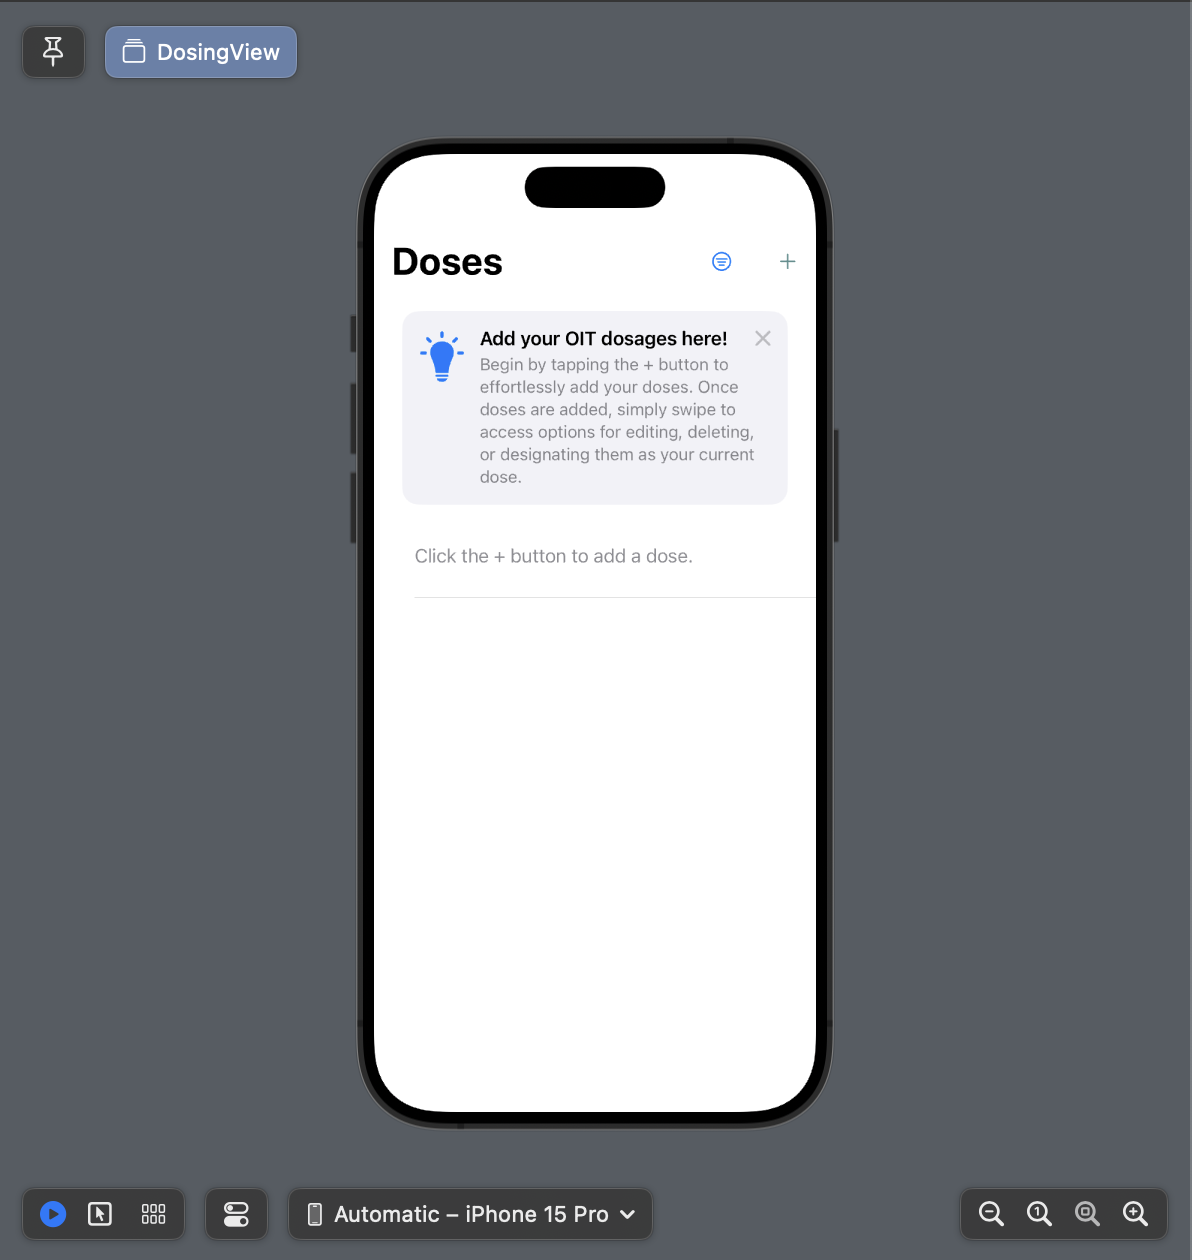
\includegraphics[width=0.5\linewidth]{thesis//chapters//images/SwiftUICanvas.png}
    \caption{SwiftUI Canvas}
    \label{fig:swiftUICanvas}
\end{figure}

\begin{figure} [H]
    \centering
    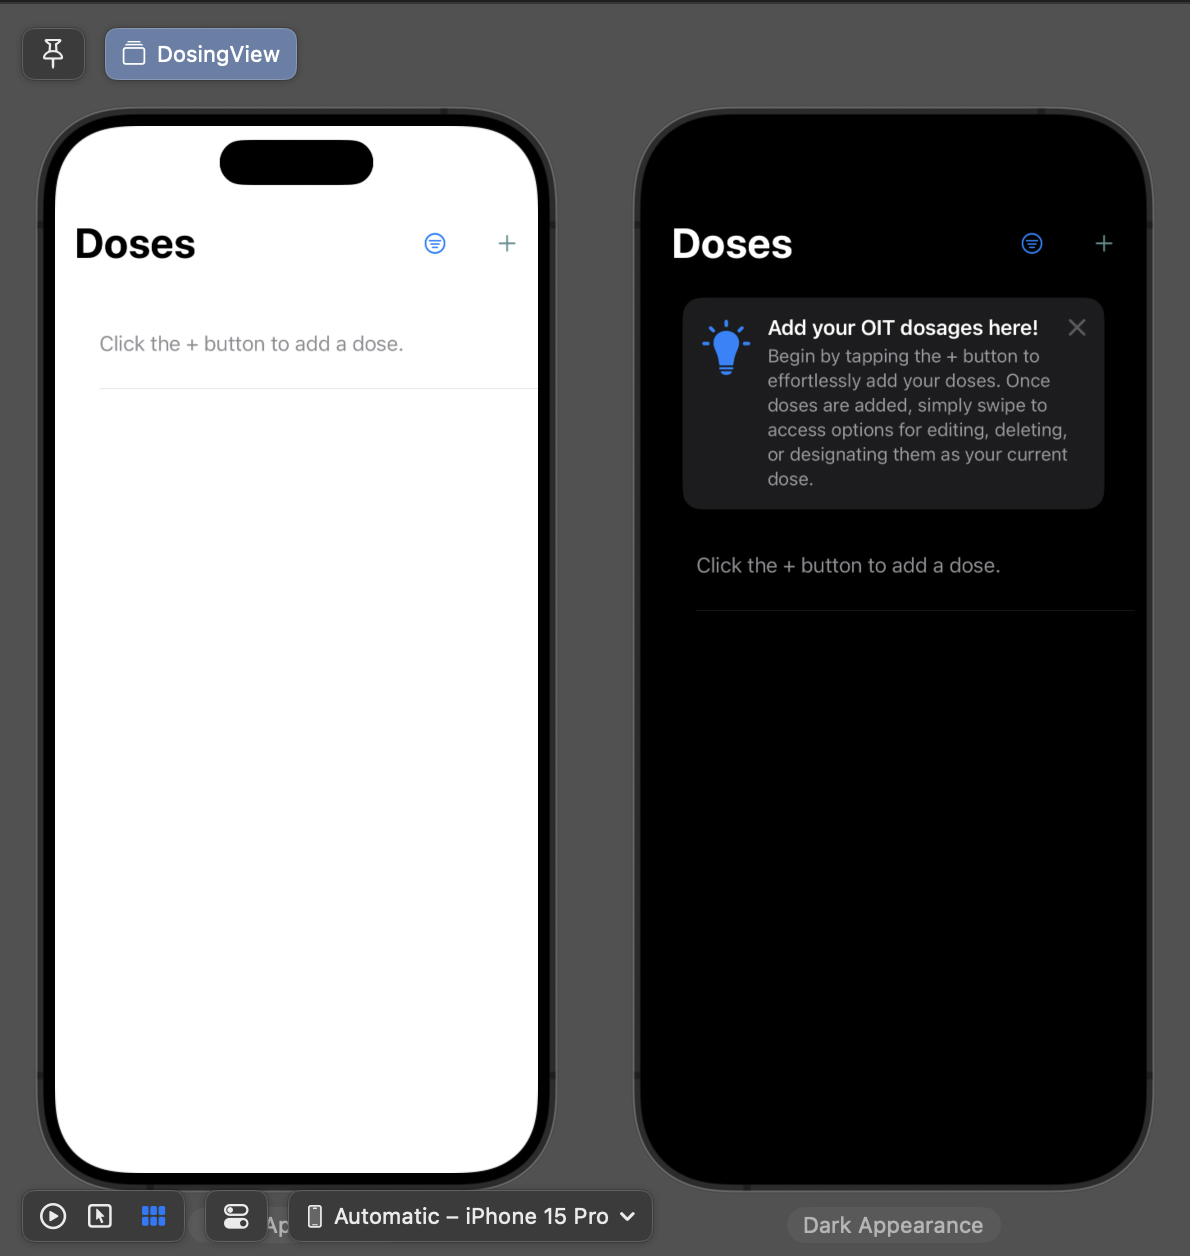
\includegraphics[width=0.5\linewidth]{thesis//chapters//images/SwiftUICanvasColorSchemeVariants.png}
    \caption{Swift UI Canvas Color Scheme Variants}
    \label{fig:swiftUICanvasColorVar}
\end{figure}

\begin{figure} [H]
    \centering
    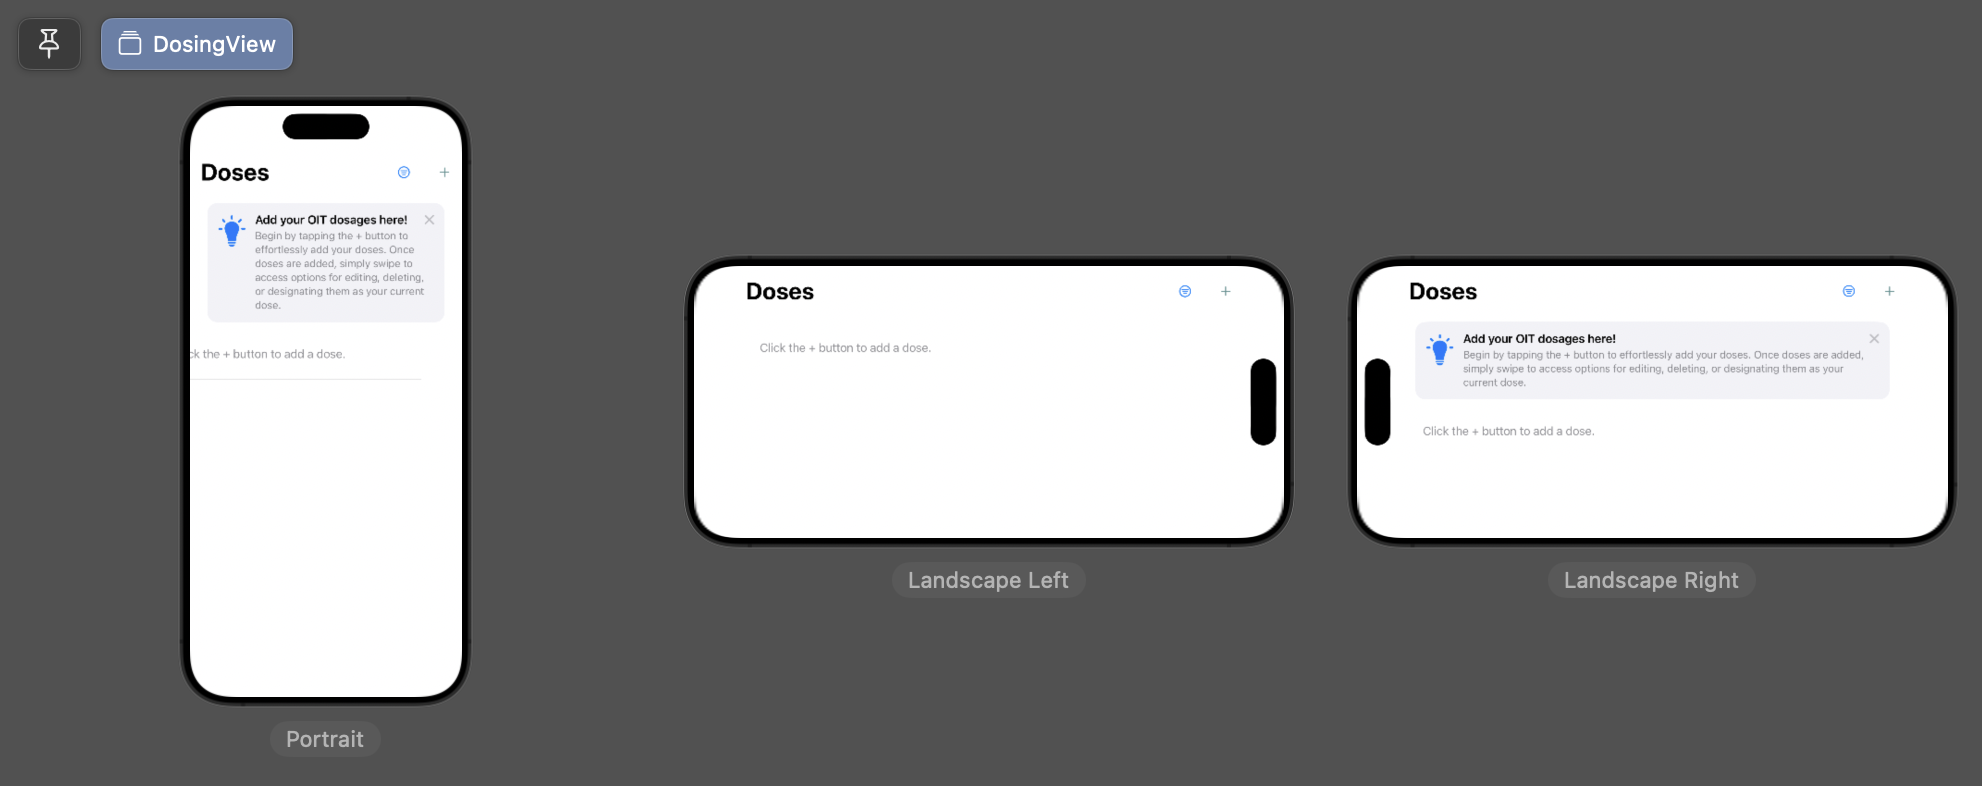
\includegraphics[width=1\linewidth]{thesis//chapters//images/SwiftUICanvasOrientationVariants.png}
    \caption{Swift UI Canvas Orientation Variants}
    \label{fig:swiftUICanvasOrientationVar}
\end{figure}

\begin{figure} [H]
    \centering
    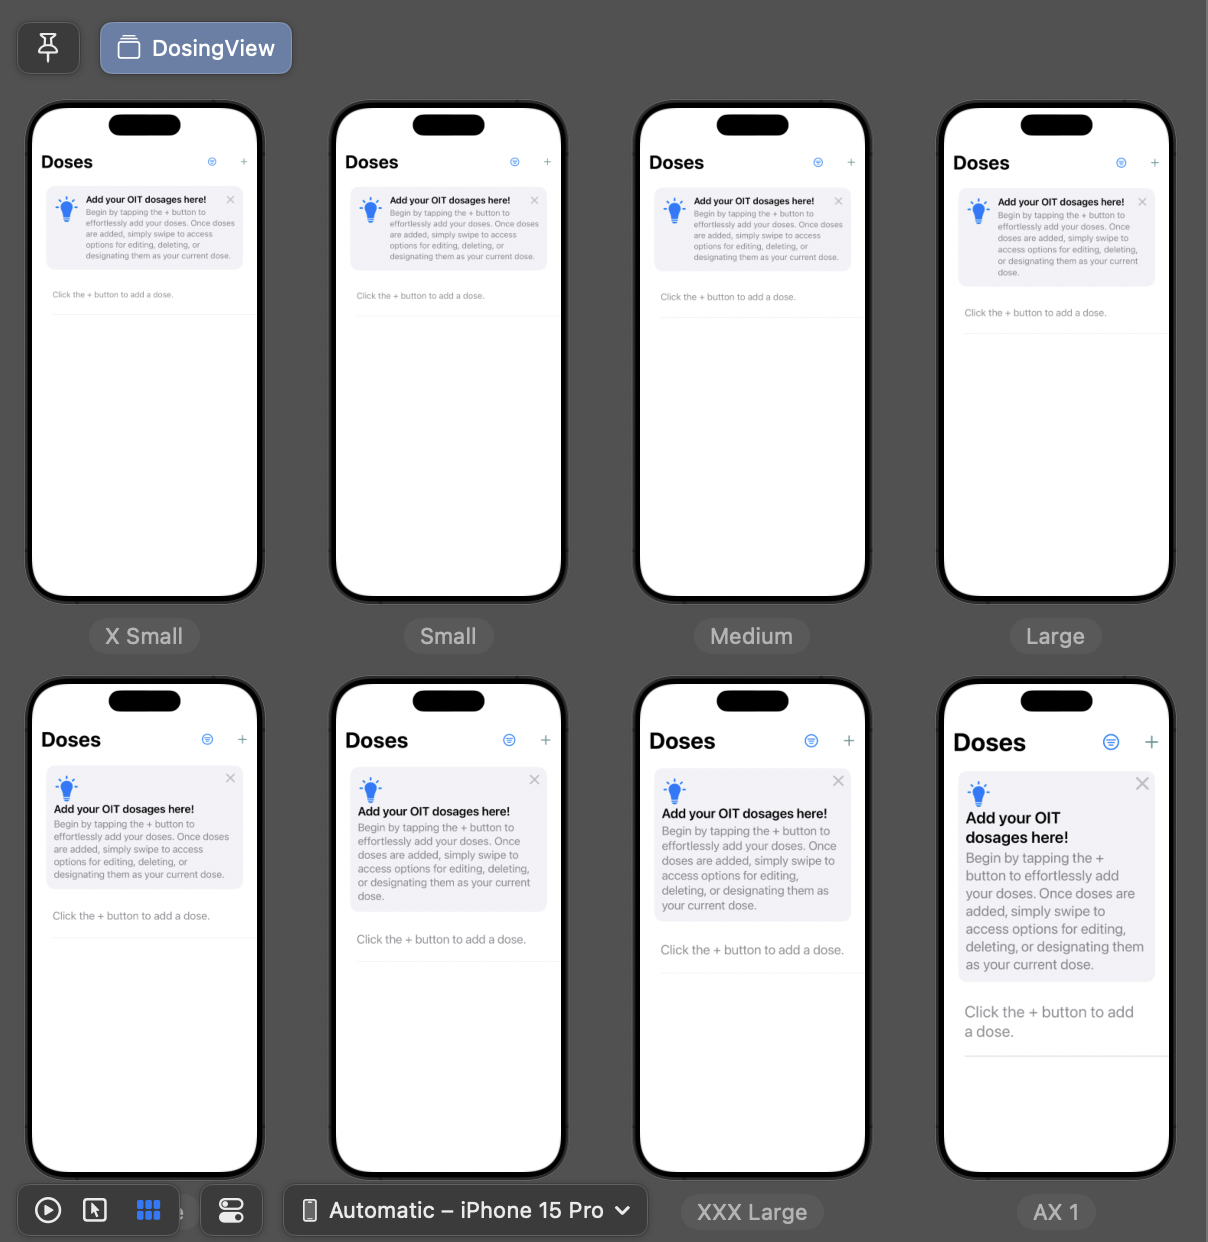
\includegraphics[width=0.75\linewidth]{thesis//chapters//images/SwiftUIDynamicTypeVariants.png}
    \caption{Swift UI Canvas Dynamic Type Variants}
    \label{fig:swiftUICanvasDTVar}
\end{figure}

\begin{figure} [H]
    \centering
    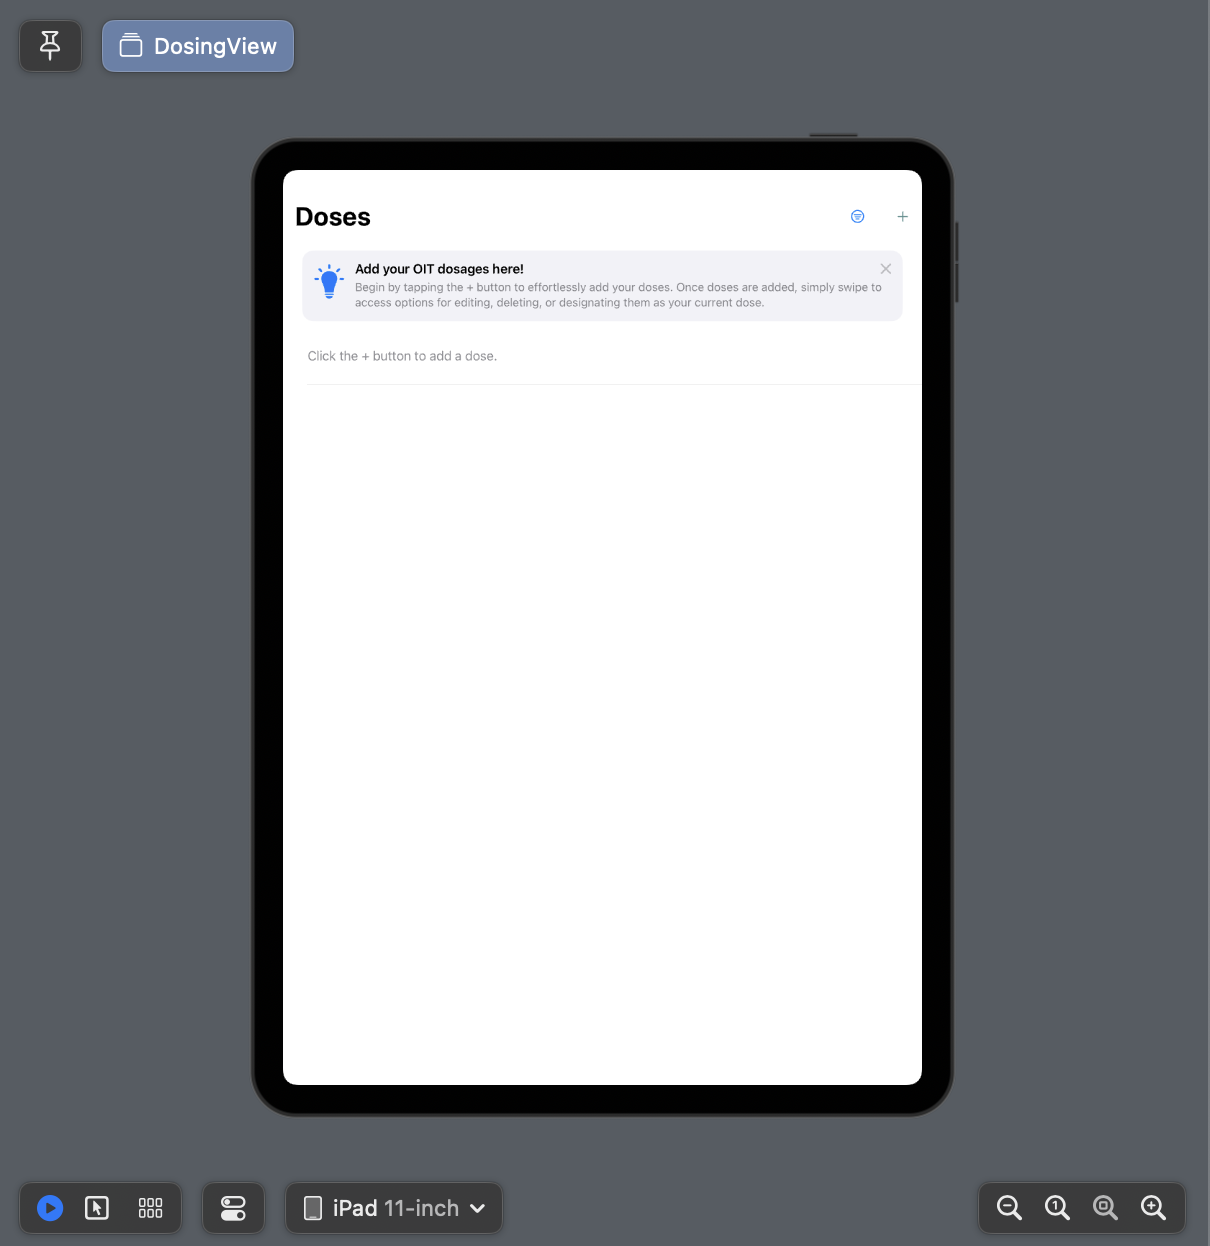
\includegraphics[width=0.75\linewidth]{thesis//chapters//images/SwiftUIDeviceVariant.png}
    \caption{Swift UI Canvas Device Variant}
    \label{fig:deviceVar}
\end{figure}

Additionally, I deployed the application onto my own phone and simulator devices, in order to test the UI in a real world scenario. This was a very helpful way to test the UI and visuals, as certain issues only replicated on device and didn't show up in the Xcode previews.

By conducting comprehensive visual testing, I aimed to guarantee a visually cohesive and appealing user experience.

\section{XCTests and XCUITests}

XCTests and XCUITests served as integral tools for validating the functional aspects of the application throughout its development. These testing frameworks facilitated the creation and execution of unit tests, ensuring the reliability and correctness of the underlying codebase. Regularly running XCTests enabled me to catch and address potential bugs or regressions early in the development process, contributing to the overall stability of the app. Additionally, the use of XCUITests allowed for the automated testing of the app's user interface, simulating user interactions and verifying the correct behavior of UI components.

\section{User Testing}

The user testing phase involved a personalized and hands-on approach to evaluating the application's practical utility.

As a patient undergoing daily maintenance doses of Oral Immunotherapy, I immersed myself in the user experience by utilizing the app in my daily routine. This enabled me to assess the real-world applicability of the application, focusing on aspects such as ease of use, convenience, and the integration of the app into my daily life. Throughout this process, I meticulously logged doses and symptoms, providing valuable insights into the app's functionality and user-friendlines

Although I didn't conduct a formal user study with other users, I did thoroughly design a study below, which could be implemented as a next step.

\subsection{User Study}

To extend the evaluation of the Oral Immunotherapy application beyond individual testing, a formal user study is proposed. The study aims to gather diverse feedback from a representative user population, ensuring a comprehensive understanding of the app's usability, effectiveness, and overall user satisfaction.

\subsubsection{Objectives}

The primary objectives of the user study are as follows:

\begin{itemize}
    \item \textbf{Usability Assessment:} Evaluate the ease of use and user-friendliness of the application, focusing on navigation, feature discoverability, and overall interaction.
    \item \textbf{Effectiveness Evaluation:} Assess the effectiveness of the app in aiding users with daily maintenance doses of Oral Immunotherapy, emphasizing its ability to provide accurate information, timely reminders, and useful insights.
    \item \textbf{Integration into Daily Life: }Examine how well the application integrates into users' daily routines and lifestyles, considering factors such as convenience, time efficiency, and overall impact on their oral immunotherapy management.
    \item \textbf{Feedback Collection:} Gather qualitative and quantitative feedback from participants to identify strengths, weaknesses, and areas for improvement in the application
\end{itemize}

\subsubsection{Participant Recruitment}

Participants for the user study will be recruited from the target user demographic of individuals undergoing oral immunotherapy. Recruitment will aim for diversity in age, technological proficiency, and length of time they have been undergoing oral immunotherapy.

\subsubsection{Methodology}

The user study will adopt a mixed-methods approach, combining quantitative surveys and qualitative interviews to provide a comprehensive assessment.

\begin{itemize}
    \item \textbf{Pre-Study Questionnaire:} Participants will complete a pre-study questionnaire to gather baseline information, including demographics, technological proficiency, and any prior experience with oral immunotherapy management apps.
    \item \textbf{Task-based Testing:} Participants will be given a set of predefined tasks within the application to perform. These tasks will cover essential functionalities, such as setting up their account, logging doses, and accessing relevant information.
    \item \textbf{Post-Task Surveys:} After completing each task, participants will provide feedback through structured surveys, rating their experience based on predefined criteria.
    \item \textbf{Interviews:} A subset of participants will be selected for in-depth interviews to explore their overall impressions, challenges encountered, and suggestions for improvement. These interviews will provide qualitative insights into user experiences and perceptions.
\end{itemize}

\subsubsection{Data Analysis}

Quantitative data from surveys will be analyzed using statistical tools to derive overall performance metrics and identify patterns. Qualitative data from interviews will be analyzed thematically to uncover nuanced feedback and user narratives.

\subsection{Conclusion}

While my personal testing provided valuable insights, the proposed user study is designed to offer a more extensive and diverse evaluation of the Oral Immunotherapy application. Implementing this study as the next step will not only enhance the application's refinement based on collective user feedback but also contribute to its broader acceptance and effectiveness within the target user population.